%%%%%%%%%%%%%%%%%%%%%%%%%%%%%%%%%%%%%%%%%%%%%%%%%%%%%%%%%%%%%%%%%%%%%%%%
%% Nonconvex A3 Coxeter-Chamber Atlas
%% Public release-candidate manuscript; publication remains owner-gated.
%%%%%%%%%%%%%%%%%%%%%%%%%%%%%%%%%%%%%%%%%%%%%%%%%%%%%%%%%%%%%%%%%%%%%%%%
\documentclass[11pt,a4paper]{amsart}
\pdfinfoomitdate=1
\pdfsuppressptexinfo=-1
\pdftrailerid{}

\usepackage[T1]{fontenc}
\usepackage[utf8]{inputenc}
\usepackage[english]{babel}
\usepackage{lmodern}
\usepackage[protrusion=true,expansion=false]{microtype}
\usepackage{amsmath,amssymb,amsthm,mathtools}
\usepackage{booktabs,array,enumitem,longtable,graphicx}
\usepackage{xurl}
\usepackage[hidelinks]{hyperref}
\usepackage[nameinlink,capitalise,noabbrev]{cleveref}
\setlength{\emergencystretch}{3em}
\raggedbottom
\Urlmuskip=0mu plus 2mu\relax

\newtheorem{theorem}{Theorem}[section]
\newtheorem{lemma}[theorem]{Lemma}
\newtheorem{proposition}[theorem]{Proposition}
\newtheorem{corollary}[theorem]{Corollary}
\newtheorem{problem}[theorem]{Problem}
\theoremstyle{definition}
\newtheorem{definition}[theorem]{Definition}
\newtheorem{algorithm}[theorem]{Algorithm}
\theoremstyle{remark}
\newtheorem{remark}[theorem]{Remark}

\DeclareMathOperator{\Stab}{Stab}
\DeclareMathOperator{\Aut}{Aut}
\DeclareMathOperator{\Iso}{Iso}
\DeclareMathOperator{\can}{can}
\newcommand{\T}{\mathcal T}
\newcommand{\C}{\mathcal C}
\newcommand{\Orb}{\mathcal O}
\newcommand{\G}{\mathfrak S_4}
\newcommand{\A}{\mathfrak A_4}
\newcommand{\Om}{\Omega}
\newcommand{\kk}{\kappa}
\newcommand{\id}{\mathrm{id}}
\newcommand{\bits}[1]{\mathtt{#1}}
\newcommand{\rowid}[1]{\texttt{#1}}
\newcommand{\code}[1]{\texttt{#1}}
\newcommand{\abs}[1]{\lvert#1\rvert}
\newcommand{\set}[1]{\{#1\}}

\crefname{lemma}{Lemma}{Lemmas}
\Crefname{lemma}{Lemma}{Lemmas}
\crefname{corollary}{Corollary}{Corollaries}
\Crefname{corollary}{Corollary}{Corollaries}
\crefname{proposition}{Proposition}{Propositions}
\Crefname{proposition}{Proposition}{Propositions}
\crefname{algorithm}{Algorithm}{Algorithms}
\Crefname{algorithm}{Algorithm}{Algorithms}


\hypersetup{
  pdftitle={The Nonconvex A3 Coxeter-Chamber Atlas},
  pdfauthor={Oleksiy Babanskyy},
  pdfsubject={congruence rigidity and finite classification of nonconvex Coxeter-pure tetrahedral tilings},
  pdfkeywords={Coxeter complex, regular tetrahedron, exact cover, symmetric group, Patterson function, homometry, congruent dissection}
}

\title[The nonconvex $A_3$ chamber atlas]
{The Nonconvex $A_3$ Coxeter-Chamber Atlas:\\
Congruence Rigidity, Exact Covers, and Patterson Separation}
\author{Oleksiy Babanskyy}
\date{}

\begin{document}
\begin{abstract}
The barycentric $A_3$ dissection of a regular tetrahedron consists of $24$
orthoscheme chambers naturally indexed by $S_4$.  Earlier work classified the
$15$ connected convex Coxeter-pure tiling orbits, reported an exhaustive audit
count of $82$ connected nonconvex left-translate tiling orbits, and posed the
classification of nonconvex congruent tilers as an open problem.  We close
that problem within the fixed Coxeter-pure carrier.  On all $2{,}874$ eligible
connected chamber-union orbits, an exact rank-three corner-locus audit proves
that free Euclidean congruence is precisely left $S_4$ equivalence.  Hence
congruent Coxeter-pure covers are exactly left-translate covers.  We then
construct the complete canonical atlas behind the earlier count and determine
its cover, contact, and symmetry structure.

The $82$ nonconvex orbits have chamber sizes $6,8,12$, with multiplicities
$14,18,50$.  The element-labelled right Patterson function
$a_U(h)=\abs{U\cap Uh}$ separates all atlas rows, whereas three natural
compressions yield only $20$, $33$, and $32$ classes.  We enumerate $786$
exact covers, $86$ cover orbits, $1{,}148$ multiplier selectors, and $102$
selector orbits; every selector-independent carrier is a typed double coset.
Rank-coloured contact complexes distinguish information invisible to their
rank marginals and produce two certified local-to-global obstruction pairs.
The atlas has $82$ full and $159$ oriented tile-congruence classes; its $86$
partition classes split into $151$ oriented classes, all are tile-transitive
inside the tetrahedron, and $69$ are rotation-tile-transitive.  Every result is
an exact finite statement for the fixed $A_3$ carrier: every partition member
is a union of its chambers.  The previously published count $15+82$ is prior
art and a replay target, not a novelty claim.

\end{abstract}
\maketitle

\noindent\textbf{Keywords.}
Coxeter complex; regular tetrahedron; congruent dissection; exact cover;
symmetric group; Patterson function; homometry; coloured flag complex.

\smallskip
\noindent\textbf{MSC 2020.}
Primary: 52C20, 05B45. Secondary: 20B30, 05E18, 52B15.

\tableofcontents

\section{Introduction}\label{sec:introduction}

\subsection{From the convex catalogue to the nonconvex atlas}

The barycentric subdivision of a regular tetrahedron is simultaneously a
geometric dissection into $24$ congruent orthoschemes and the spherical
Coxeter complex of type $A_3$ coned to the barycentre.  This coincidence
makes a finite classification possible: unions of chambers become subsets of
$S_4$, adjacency is a Cayley-graph relation, and tetrahedral relabelling is
left multiplication.  The finite model is small enough for exhaustive
enumeration but large enough for nonconvexity, multiple exact covers,
chirality, and contact phenomena that do not occur in the convex catalogue.

The convex theory was developed in \cite{BabanskyyT2}.  There, connected
convex chamber unions were identified with poset cones, and the tiling pieces
were classified by the $15$ series--parallel poset types on four elements.
The same project reported an independent exhaustive count
\[
  97=15+82
\]
of connected left-translate tiling orbits, with $82$ nonconvex rows, and
posed the classification of connected nonconvex chamber unions that tile by
congruent copies as an open problem.  The numerical split is therefore
self-prior-art.  The purpose of this paper is to close the congruence gap
left by that audit and replace the bare count by a canonical, structurally
complete, and independently replayable atlas.

Four questions drive the construction.
\begin{enumerate}[label=(\roman*),leftmargin=2.2em]
\item Does free Euclidean congruence enlarge a left $S_4$ orbit anywhere in
the complete eligible chamber-union carrier?
\item Can the $82$ rows be separated by an intrinsic invariant that respects
the locked tetrahedral action?
\item How many inequivalent exact covers does each tile admit, and what is the
algebraic structure of its multiplier choices?
\item Which contact and symmetry data survive after local compression, and
where do local equivalences fail to assemble globally?
\end{enumerate}

The answers use four different layers.  An all-candidate rank-three
corner-locus theorem identifies free congruence with the locked left action.
The labelled right Patterson function separates tile orbits.  Exhaustive
exact-cover and multiplier enumeration describes all partitions inside the
finite carrier.  Exact rank-coloured barycentric intersections then recover
contact, handedness, and finite-container transitivity.

\subsection{Main results}

The main theorem packages the numerical statements; precise definitions and
stronger typed formulations appear in later sections.

\begin{theorem}[Nonconvex $A_3$ chamber atlas: overview]
\label{thm:overview}
In the fixed $24$-chamber $A_3$ dissection of the regular tetrahedron, under
the action and equivalences of \cref{sec:model}, the following hold.
\begin{enumerate}[label=(\alph*),leftmargin=2.2em]
\item There are exactly $82$ free-congruence classes of connected
halfspace-nonconvex pieces that tile by congruent Coxeter-pure copies.  Every
such copy is a left $S_4$ translate.  Their chamber sizes are $6,8,12$, with
multiplicities $14,18,50$.
\item The full element-labelled right Patterson vector separates the $82$
orbits.  Conjugacy-class sums, within-class coordinate multisets, and the
fully unlabelled coordinate multiset yield respectively $20,33,32$ classes.
\item The $82$ tiles admit $786$ exact covers in $86$ global-left cover
orbits.  Their $1{,}148$ multiplier selectors form $102$ selector orbits,
with the exact taxonomy $90+2+10$ described in \cref{sec:covers}.
\item Canonical representatives of the $86$ cover orbits have $212$
within-cover contact edges and $82$ edgewise signatures.  Two pairs are
edgewise equivalent but not globally aligned.
\item The atlas has $82$ full Euclidean and $159$ orientation-preserving tile
classes, split into $77$ chiral and $5$ achiral full classes.  The $86$
partition classes split into $151$ oriented classes; all $86$ are
finite-container tile-transitive and $69$ are rotation-tile-transitive.
\end{enumerate}
\end{theorem}

Part~(a) combines the left-exact-cover census with the independent
all-candidate rigidity theorem \cref{thm:global-rigidity}.  The latter ranges
over all $2{,}874$ eligible connected chamber-union orbits, not merely the
$82$ positive rows, and shows that every congruent Coxeter-pure cover is
already a left-translate cover; see \cref{cor:congruent-atlas}.  Here
\emph{Coxeter-pure} means that every partition member remains a union of the
fixed $A_3$ chambers.

The result in part~(b) is deliberately bounded.  Patterson functions and
homometry are classical \cite{MandereauEtAl2011,RosenblattSeymour1982,
GenuysPopoff2018}.  We prove injectivity only on the displayed $82$-row
family, not for arbitrary subsets of a finite group.  Likewise, the contact
and symmetry statements are about a finite tetrahedral container, not a
periodic monohedral tiling of Euclidean space.

\subsection{Why the labels and types matter}

Several superficially similar objects must remain distinct.  A tile orbit is
not a cover orbit; a cover is not a multiplier selector; the stabiliser of a
tile is not the stabiliser of a cover; an edgewise family of contact
equivalences is not one globally coherent equivalence.  Losing these types
creates false uniqueness and false local-to-global statements.  The paper
therefore fixes all actions, quotient relations, and quantifier orders before
stating the enumerative results.

The same discipline explains the Patterson theorem.  Left multiplication
fixes every labelled coordinate, while right multiplication conjugates the
coordinate labels.  The values alone do not suffice: all three natural label
compressions collide.  Thus the nonabelian labelling is not decorative data;
it is the separating information on this carrier.

\subsection{Logical status and organisation}

The three-way equivalence between halfspace, chamber-geodesic, and Euclidean
convexity for connected $A_3$ chamber unions is imported from
\cite{BabanskyyT2}.  All enumerations, Patterson identities, exact-cover
classifications, contact comparisons, and ambient congruence calculations in
this paper use exact integer or rational arithmetic.  The companion package
fully reconstructs the connected and eligible census, the global congruence
gate, and the congruent-copy exact-cover closure.  The Patterson, cover,
selector, contact, boundary, and ambient-symmetry layers are distributed as
exact parent-pinned snapshots with record hashes and public structural
recheckers; their production builders remain internal.  In particular, the
congruence statement is deduced only after the complete eligible carrier has
passed both exact isometry lanes.  A machine certificate supports a finite
proof; its stated replay level is part of the claim boundary and does not
enlarge the theorem's scope.

\Cref{sec:model} fixes the geometric and group-theoretic model.
\Cref{sec:finite-reduction} proves the finite reduction and constructs the
atlas.  \Cref{sec:patterson} develops the separating invariant.
\Cref{sec:covers,sec:contacts} classify covers, selectors, and contact
complexes.  \Cref{sec:ambient} treats congruence and transitivity, and
\cref{sec:boundary} records a presentation-sensitivity result.  The final
sections delimit prior art and give the replay contract.  The appendices
provide the search proof, the complete $82$-row catalogue, and a
theorem-to-certificate crosswalk.

\section{The fixed \texorpdfstring{$A_3/S_4$}{A3/S4} model}\label{sec:model}

\subsection{The tetrahedron and its Coxeter chambers}

Let
\[
 H=\left\{x\in\mathbb R^4:\sum_{i=0}^{3}x_i=1\right\},
 \qquad
 T=\operatorname{conv}\{e_0,e_1,e_2,e_3\}\subset H,
\]
with the induced Euclidean metric.  This is a regular tetrahedron of edge
length $\sqrt2$; rescaling does not affect any statement below.  For a
nonempty set $I\subseteq\{0,1,2,3\}$ put
\[
 b_I=\frac1{|I|}\sum_{i\in I}e_i.
\]
If $\sigma=\sigma_0\sigma_1\sigma_2\sigma_3$ is a one-line permutation, the
closed barycentric chamber indexed by $\sigma$ is
\[
 \Delta_\sigma=
 \operatorname{conv}\left(
 b_{\{\sigma_0\}},
 b_{\{\sigma_0,\sigma_1\}},
 b_{\{\sigma_0,\sigma_1,\sigma_2\}},
 b_{\{0,1,2,3\}}
 \right).
\]
The $24$ chambers have disjoint interiors and union $T$.

Write $G=S_4$.  We compose permutations as functions,
$(pq)(i)=p(q(i))$.  The coordinate permutation
\[
 \Phi_g(x)_i=x_{g^{-1}(i)}
\]
is an isometry of $T$ and satisfies
$\Phi_g(\Delta_\sigma)=\Delta_{g\sigma}$.  Hence the full isometry group of
$T$ is realised by left multiplication on chamber labels; its
orientation-preserving subgroup is $A_4$.

Let $s_i$ exchange positions $i$ and $i+1$ for $i=0,1,2$.  Two chambers
share a facet precisely when their labels differ by right multiplication by
one $s_i$.  The chamber graph is therefore
\[
 \Gamma=\operatorname{Cay}_{\mathrm{right}}
 (S_4,\{s_0,s_1,s_2\}).
\]
Left multiplication is a graph automorphism because
$g(\sigma s_i)=(g\sigma)s_i$.

\begin{figure}[ht]
\centering
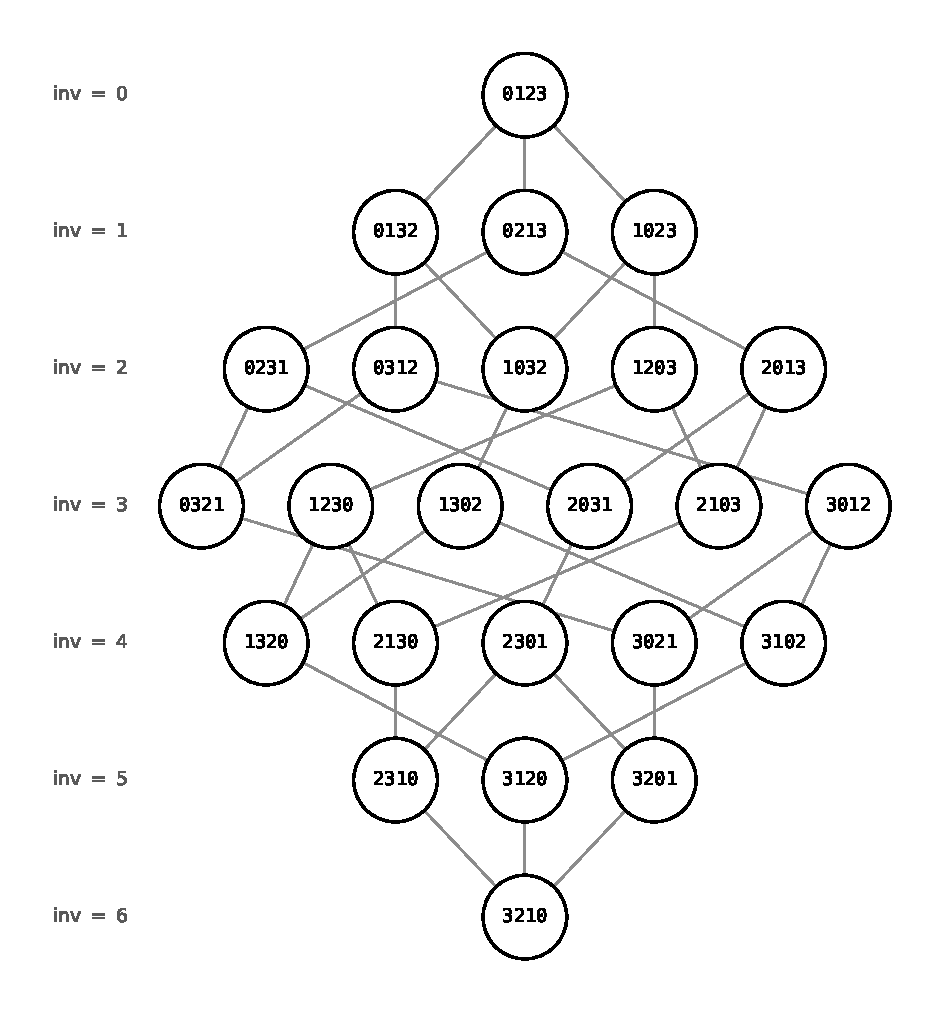
\includegraphics[width=.72\textwidth]{figures/a3_chamber_graph.pdf}
\caption{The $24$ chambers and their facet-adjacency graph.  Edges are
right multiplication by an adjacent transposition; left $S_4$ acts by graph
automorphisms.  Figure reused from \cite{BabanskyyT2} under CC BY 4.0.}
\label{fig:chamber-graph}
\end{figure}

\subsection{Pieces, masks, and convexity}

\begin{definition}[Coxeter-pure piece]
A piece is a nonempty subset $U\subseteq G$, identified with the closed
polyhedron
\[
 |U|_T=\bigcup_{\sigma\in U}\Delta_\sigma.
\]
It is \emph{connected} when the induced chamber graph $\Gamma[U]$ is
connected.  This is facet-connectedness; contact through only an edge or a
vertex does not suffice.
\end{definition}

Order the $24$ words lexicographically and let $\operatorname{idx}(\sigma)$
be the zero-based position.  The integer mask
\[
 m(U)=\sum_{\sigma\in U}2^{\operatorname{idx}(\sigma)}
\]
is the primary exact encoding.  All masks in the paper are displayed as six
hexadecimal digits.

For $i,j\in\{0,1,2,3\}$ define $i<_{U}j$ when $i$ precedes $j$ in every word
of $U$.  These unanimous precedence relations define a poset $P_U$.  Its set
of linear extensions is the halfspace closure
\[
 \operatorname{hcl}(U)=L(P_U).
\]
We call $U$ halfspace-convex when $U=\operatorname{hcl}(U)$ and
halfspace-nonconvex otherwise.  For connected pieces this agrees with
chamber-geodesic and Euclidean convexity by the three-way theorem of
\cite{BabanskyyT2}.  The computation uses the halfspace predicate; the
geometric terminology invokes that theorem with its stated hypotheses.

\subsection{Four typed equivalences}

\begin{definition}[Tile orbit]
The left tile orbit and stabiliser of $U$ are
\[
 \Orb_L(U)=\{gU:g\in G\},
 \qquad H_U=\Stab_L(U)=\{g\in G:gU=U\}.
\]
Two pieces are \emph{left-tile equivalent} when they lie in the same
$\Orb_L$ orbit.  The canonical representative is
\[
 \can_L(U)=\arg\min_{V\in\Orb_L(U)}m(V).
\]
The minimum is numeric bitmask order, not lexicographic order on word lists.
\end{definition}

\begin{definition}[Exact cover]
An exact left-translate cover of $U$ is an unordered set
\[
 \C=\{g_1U,\ldots,g_rU\}\subseteq\Orb_L(U)
\]
whose chamber sets are pairwise disjoint and whose union is $G$.  Necessarily
$r=24/|U|$.  Covers $\C$ and $\C'$ are \emph{cover equivalent} when
$\C'=g\C:=\{gV:V\in\C\}$ for one $g\in G$.
\end{definition}

\begin{definition}[Selector]
A multiplier selector for a cover $\C$ of $U$ is a set $A\subseteq G$ such
that
\[
 \C=\{aU:a\in A\}.
\]
Selectors are not unique when $H_U$ is nontrivial.  Their natural global-left
action is $A\mapsto gA$.
\end{definition}

\begin{definition}[Free congruence]
Pieces $U,V$ are \emph{freely congruent} if an affine Euclidean isometry of
$H$ maps $|U|_T$ onto $|V|_T$.  This does not, by definition, require the
isometry to preserve the ambient tetrahedron.  Whole partitions are
congruent when one isometry of $H$ maps the complete unordered family of
pieces onto the other.
\end{definition}

\begin{definition}[Congruent Coxeter-pure cover]
A congruent Coxeter-pure cover is an unordered family
$\{U_1,\ldots,U_r\}$ of connected pieces in the fixed chamber carrier whose
polyhedral interiors are pairwise disjoint, whose union is $T$, and whose
members are pairwise freely congruent.  Thus every member is itself a union
of chambers of the fixed $A_3$ dissection.  This is the finite-carrier
meaning of \emph{by congruent copies} used in the Coxeter-pure problem;
copies whose boundaries cut chamber interiors are outside the definition.
\end{definition}

The first three definitions are finite group actions.  Free congruence is a
geometric relation and must be compared with them rather than identified by
notation.  Right multiplication is also distinct: it conjugates the
adjacent-transposition generating set and need not preserve connectivity.

\begin{lemma}[Basic covariance]\label[lemma]{lem:basic-covariance}
Left multiplication preserves chamber adjacency, cardinality, halfspace
closure, exact-cover incidence, and Euclidean shape.  Moreover
\[
 |\Orb_L(U)|=\frac{24}{|H_U|}.
\]
\end{lemma}
\begin{proof}
Adjacency covariance was observed above.  Relabelling the ground set carries
the precedence poset $P_U$ to $P_{gU}$, so it carries their linear extensions
and halfspace closures.  The other assertions follow from the coordinate
isometry $\Phi_g$, and the final identity is orbit--stabiliser.
\end{proof}

\section{Finite reduction and the canonical atlas}
\label{sec:finite-reduction}

\subsection{Candidate space}

There are $2^{24}-1$ nonempty chamber masks.  A tiler must be connected and
its cardinality must divide $24$.  We first enumerate connected masks, apply
the divisibility filter, and then retain one numeric-minimum representative
from each left $S_4$ orbit.  The reduction is summarised in
\cref{tab:reduction}.

\begin{table}[ht]
\centering
\caption{Exact finite reduction.  ``Eligible'' means connected with chamber
cardinality dividing $24$.}
\label{tab:reduction}
\begin{tabular}{@{}lr@{}}
\toprule
stage & count\\
\midrule
connected nonempty masks & $1{,}210{,}648$\\
eligible connected masks & $67{,}681$\\
canonical eligible left-orbit representatives & $2{,}874$\\
exact left-translate tilers & $97$\\
exact-cover negatives & $2{,}777$\\
convex/nonconvex tiler split & $15/82$\\
\bottomrule
\end{tabular}
\end{table}

\begin{lemma}[Canonical reduction]\label[lemma]{lem:canonical-reduction}
Every connected piece is left-equivalent to exactly one stored canonical
mask.  A canonical piece is a left-translate tiler if and only if the
exact-cover recursion below returns a cover.
\end{lemma}
\begin{proof}
The finite orbit $\{gU:g\in S_4\}$ has a unique minimum integer mask.  Left
multiplication preserves adjacency by \cref{lem:basic-covariance}.  Every
cover of any orbit member translates to a cover of the canonical member, and
conversely.  It therefore remains only to show that the recursion enumerates
all covers, which is \cref{lem:exact-cover-completeness} below.
\end{proof}

\subsection{Exact-cover search}

For a fixed canonical $U$, let $\mathcal O$ be the set of distinct masks in
$\Orb_L(U)$.  A search state is a pair $(R,\mathcal F)$, where $R$ is the
remaining uncovered mask and $\mathcal F$ is the chosen family.  Initially
$R=G$ and $\mathcal F=\varnothing$.  At a nonterminal state choose the
least-indexed chamber $c$ of $R$ and branch over all $V\in\mathcal O$ with
$c\in V\subseteq R$.

\begin{algorithm}[Least-uncovered exact-cover recursion]
\label[algorithm]{alg:exact-cover}
\begin{enumerate}[leftmargin=2.2em]
\item If $R=\varnothing$, output $\mathcal F$.
\item Let $c$ be the least chamber contained in $R$.
\item For every $V\in\mathcal O$ with $c\in V$ and $V\cap(G\setminus R)
=\varnothing$, recurse on $(R\setminus V,\mathcal F\cup\{V\})$.
\end{enumerate}
\end{algorithm}

\begin{lemma}[Exact-cover completeness]\label[lemma]{lem:exact-cover-completeness}
\Cref{alg:exact-cover} outputs every unordered exact cover of $G$ by members
of $\Orb_L(U)$ exactly once.
\end{lemma}
\begin{proof}
Let $\C$ be an exact cover extending the current partial family.  The least
uncovered chamber $c$ belongs to a unique member $V$ of $\C$.  That member is
one of the algorithm's branches, so induction on the number of uncovered
chambers reaches $\C$.  Conversely, each branch adds a subset of the remaining
mask, hence every terminal family is disjoint and covers $G$.  Choosing the
least uncovered chamber makes the sequence of chosen members canonical for
an unordered cover, so no cover is output twice.
\end{proof}

Two independent implementations support the enumeration.  The source-replay
lane executes the earlier T2 algorithms at their pinned revision.  The
independent lane scans all nonempty $24$-bit masks, reconstructs the chamber
graph, halfspace closure, orbit canonicalisation, and exact-cover recursion
without importing the T2 code.  The two lanes agree on the entire $97$-row
positive stream and its exact digest.

\subsection{The atlas theorem}

\begin{theorem}[Canonical nonconvex left-translate atlas]
\label{thm:left-atlas}
Up to left $S_4$ equivalence, exactly $82$ connected
halfspace-nonconvex pieces tile the reference tetrahedron by left translates.
Their distribution is
\[
\begin{array}{c|ccc}
|U|&6&8&12\\ \hline
\#\text{ orbits}&14&18&50.
\end{array}
\]
Together with the $15$ convex types of \cite{BabanskyyT2}, they exhaust the
$97$ positive canonical representatives in \cref{tab:reduction}.
\end{theorem}
\begin{proof}
By \cref{lem:canonical-reduction,lem:exact-cover-completeness}, the exhaustive
candidate scan and exact-cover recursion decide every eligible left orbit.
Both implementations find the same $2{,}777$ negatives and $97$ positives.
The halfspace predicate, calibrated against the imported three-way convexity
theorem on connected masks, divides the positives into $15$ convex and $82$
nonconvex rows.  Grouping the latter by popcount gives $14,18,50$.
\end{proof}

\begin{figure}[ht]
\centering
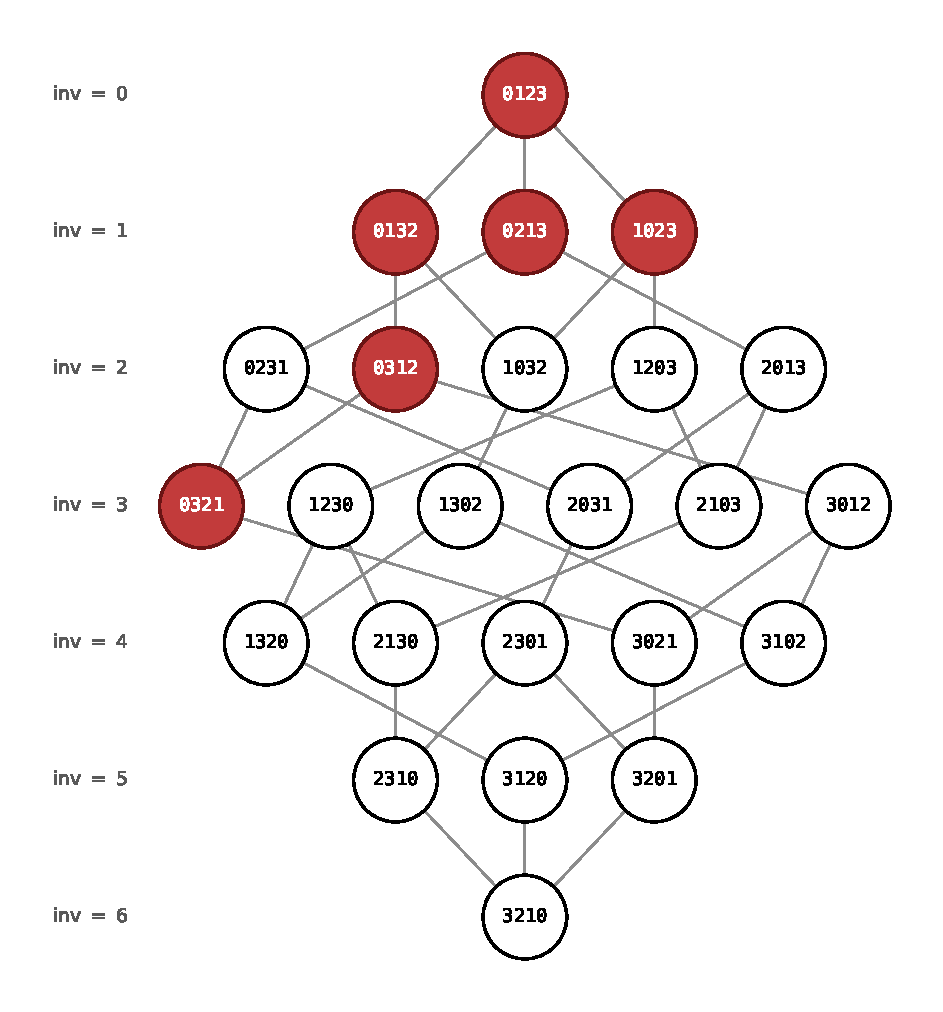
\includegraphics[width=.72\textwidth]{figures/t2_nonconvex_example.pdf}
\caption{The chamber set of the six-chamber row
\rowid{P18-NC-K06-M000077}, highlighted in the $A_3$ chamber graph.  This
was the existence witness used to show that the nonconvex problem is
nonempty in \cite{BabanskyyT2}; here it is one row of the complete atlas.
Figure reused under CC BY 4.0.}
\label{fig:nonconvex-example}
\end{figure}

Every atlas row has the content-addressed identifier
\[
 \rowid{P18-NC-K}\,|U|\,\rowid{-M}\,m(U),
\]
with the cardinality written in two decimal digits and the mask in six
uppercase hexadecimal digits.  For example, the first row is
\rowid{P18-NC-K06-M00006F}.  Source-array positions are locators, never row
identity.  The complete table appears in \cref{app:catalogue}.

\subsection{Congruence closure of the candidate universe}
\label{sec:congruence-closure}

The left-translate census is only the combinatorial half of the earlier
congruent-copy problem.  The missing implication is global: a
left-exact-cover negative must not become positive by using congruent
Coxeter-pure pieces drawn from several left orbits.  It would be circular to
check this only on the $82$ already selected rows.

The ambient argument in \cref{sec:ambient} therefore runs on all $2{,}874$
eligible canonical candidates.  \Cref{thm:global-rigidity} proves that free
Euclidean congruence equals left $S_4$ equivalence throughout that carrier,
and \cref{cor:congruent-atlas} promotes \cref{thm:left-atlas} to the complete
classification by congruent Coxeter-pure copies.  No equivalence is assumed
in the exact-cover search itself.

\section{The element-labelled Patterson separator}
\label{sec:patterson}

\subsection{Right differences in the group ring}

For $U\subseteq G$ write $X_U=\sum_{u\in U}u$ in the integral group ring
$\mathbb Z[G]$, and let $X_U^{(-1)}=\sum_{u\in U}u^{-1}$.  The coefficient of
$h$ in $X_U^{(-1)}X_U$ is
\[
 a_U(h)=|U\cap Uh|=\#\{(u,v)\in U^2:u^{-1}v=h\}.
\]
This is the right interval content, or right Patterson function, in counting
measure.  The left/right distinction is essential in a nonabelian group
\cite{MandereauEtAl2011,GenuysPopoff2018}.

\begin{lemma}[Patterson identities]\label[lemma]{lem:patterson-identities}
For $U\subseteq G$ and $g,h\in G$,
\begin{align*}
a_U(e)&=|U|,&
\sum_{h\in G}a_U(h)&=|U|^2,&
a_U(h)&=a_U(h^{-1}),\\
a_{gU}(h)&=a_U(h),&
a_{Ug}(h)&=a_U(ghg^{-1}),&
a_{G\setminus U}(h)&=|G|-2|U|+a_U(h).
\end{align*}
\end{lemma}
\begin{proof}
The first identity counts diagonal pairs, the second all ordered pairs in
$U^2$, and inversion exchanges $(u,v)$ with $(v,u)$.  In a left translate,
$(gu)^{-1}(gv)=u^{-1}v$.  In a right translate,
$(ug)^{-1}(vg)=g^{-1}u^{-1}vg$, which gives the displayed conjugation after
renaming the argument.  Finally, expand the two complement indicators in
$\sum_x(1-1_U(x))(1-1_U(xh^{-1}))$.
\end{proof}

The formula for right translation explains why coordinate labels cannot be
discarded casually.  Left translation fixes the vector pointwise; right
translation permutes it through inner automorphisms.

\subsection{Three controlled compressions}

Let $C_1,\ldots,C_5$ be the conjugacy classes of $S_4$.  We compare four
fingerprints:
\begin{enumerate}[label=(\roman*),leftmargin=2.2em]
\item the full labelled vector $(a_U(h))_{h\in G}$ in the fixed word order;
\item the five conjugacy-class sums
$\bigl(\sum_{h\in C_i}a_U(h)\bigr)_i$;
\item the ordered five-tuple of multisets
$\bigl(\{a_U(h):h\in C_i\}_{\mathrm{multi}}\bigr)_i$;
\item the single unlabelled multiset
$\{a_U(h):h\in G\}_{\mathrm{multi}}$.
\end{enumerate}
These are distinct declared quotients of the data, not interchangeable
notions of Patterson equivalence.

\begin{theorem}[Labelled Patterson separation]\label{thm:patterson}
On the $82$ rows of \cref{thm:left-atlas}, the full element-labelled right
Patterson vector is injective.  The four fingerprints above yield
\[
\begin{array}{c|cccc}
&\text{full labelled}&\text{class sums}&\text{class multisets}&
\text{unlabelled}\\ \hline
\#\text{ classes}&82&20&33&32.
\end{array}
\]
The $24$ stored coordinates occupy $17$ orbits under inversion.
\end{theorem}
\begin{proof}
For every row the $24$ coefficients are computed by exact integer
intersection.  Equality grouping gives $82$ full vectors and, after applying
each displayed quotient, $20,33,32$ classes.  The identities of
\cref{lem:patterson-identities} are checked in all $82\cdot24=1{,}968$
left-translation cases.  Inversion fixes the identity, the six
transpositions, and the three double transpositions; the other $14$ elements
form seven inverse pairs.  Thus there are $10+7=17$ inversion positions.
\end{proof}

\begin{remark}[Scope]
The theorem is a collision-free certificate on one finite family.  It is not
a phase-retrieval theorem and does not assert that second-order
autocorrelation separates arbitrary subsets of $S_4$, still less arbitrary
finite groups.  Higher-order invariants can be complete under hypotheses
where second-order data are not \cite{Kakarala2012,RadcliffeScott2007}.
\end{remark}

\subsection{The half-size complement ambiguity}

For $|U|=|G|/2$, \cref{lem:patterson-identities} gives
$a_{G\setminus U}=a_U$.  This universal ambiguity does not produce a second
atlas row in the $K12$ family.

\begin{lemma}[Complement absorption]\label[lemma]{lem:complement}
For every one of the $50$ atlas rows with $|U|=12$, the complement
$G\setminus U$ belongs to the same left tile orbit as $U$.
\end{lemma}
\begin{proof}
Every such row has a two-piece left-translate cover
$G=g_1U\sqcup g_2U$.  Multiplication by $g_1^{-1}$ gives
$G=U\sqcup gU$, where $g=g_1^{-1}g_2$.  Hence $G\setminus U=gU$.
The certificate additionally checks the relation directly for all $50$
canonical masks.
\end{proof}

The convex catalogue admits a compact separating contact vector
\cite{BabanskyyT2}.  In the nonconvex atlas, the full right-difference labels
play the parallel role.  The compression profile $82/20/33/32$ quantifies
exactly how much separation is lost when those labels are forgotten.

\section{All covers and multiplier selectors}\label{sec:covers}

\subsection{Cover orbits and selector fibres}

Fix an atlas row $U$ and an exact cover $\C$.  Besides the tile stabiliser
$H_U$, two further objects are needed:
\[
 K_\C=\Stab_L(\C)=\{g\in G:g\C=\C\}
\]
and the selector-independent lift
\[
 B_\C=\{g\in G:gU\in\C\}.
\]
The set of selectors realising this cover is
\[
 R_U(\C)=\{A\subseteq G:\{aU:a\in A\}=\C\}.
\]
Each piece $gU$ has multiplier fibre $gH_U$, so a selector chooses one
element from each such right coset.  In particular, selectors encode more
than the underlying geometric cover.

\begin{lemma}[Selector-independent carrier]\label[lemma]{lem:selector-carrier}
For every $A\in R_U(\C)$,
\[
 B_\C=AH_U,
 \qquad K_\C=\Stab_L(B_\C).
\]
Thus $B_\C$ depends on $U$ and $\C$, but not on the chosen section $A$.
\end{lemma}
\begin{proof}
The multipliers producing the piece $aU$ are precisely the elements of the
right coset $aH_U$.  Taking the union over $a\in A$ gives $B_\C=AH_U$.
A group element stabilises the cover if and only if it stabilises its full
preimage under the quotient map $g\mapsto gU$, proving the second identity.
\end{proof}

For each row we enumerate every exact cover by two algorithms: the recursive
search of \cref{alg:exact-cover} and direct combination testing inside the
left tile orbit.  Covers are canonicalised by
\[
 \can_G(\C)=
 \min_{g\in G}\operatorname{sort}\{m(gV):V\in\C\}.
\]
An independent Burnside computation verifies the orbit counts.  Selector
orbits over a canonical cover are computed as sections $R_U(\C)$ modulo
$K_\C$, which is equivalent to the global-left action after the cover has
been gauge-fixed.

\subsection{Complete enumeration}

\begin{theorem}[Cover and selector census]\label{thm:covers}
The $82$ atlas rows have $786$ unordered exact covers, forming $86$
global-left cover orbits.  Seventy-nine rows have one cover orbit.  The three
exceptions are
\[
\begin{array}{c|ccc}
\text{mask suffix}&\rowid{M00007D}&\rowid{M00016D}&\rowid{M001345}\\ \hline
\#\text{ cover orbits}&2&3&2.
\end{array}
\]
The $1{,}148$ multiplier selectors form $102$ global-left selector orbits.
Exactly $90$ of those orbits admit a representative that is a subgroup or a
one-sided subgroup coset; $2$ further orbits admit a genuine double-coset
representative but no subgroup/coset representative; the remaining $10$ are
residual.
\end{theorem}

\begin{table}[ht]
\centering
\caption{Cover and selector counts by tile size.}
\label{tab:cover-by-k}
\begin{tabular}{@{}rrrrr@{}}
\toprule
$|U|$ & tile rows & raw covers & cover orbits & selector orbits\\
\midrule
$6$  & $14$ & $102$ & $18$ & $24$\\
$8$  & $18$ & $144$ & $18$ & $21$\\
$12$ & $50$ & $540$ & $50$ & $57$\\
\midrule
total & $82$ & $786$ & $86$ & $102$\\
\bottomrule
\end{tabular}
\end{table}

\begin{proof}[Proof of \cref{thm:covers}]
For each row, the recursive and combination enumerators return the same
sorted cover stream.  Global-left canonicalisation produces the stated
orbit counts, and Burnside's lemma gives the same result independently.
For every cover representative, all selector sections are generated by the
right-$H_U$ fibres and quotiented by $K_\C$.  The subgroup inventory of
$S_4$ is regenerated from closure and contains exactly $30$ subgroups.
Testing every selector orbit against that inventory and against all typed
one- and two-sided cosets yields the disjoint taxonomy $90+2+10=102$.
Every equality is set equality in the $24$-element group; no heuristic
isomorphism test enters the count.
\end{proof}

The phrase ``$90$ coset selectors'' would be too strong.  The theorem says
that $90$ \emph{orbits admit} a subgroup/coset representative; other
selectors in the same orbit need not themselves be presented in that form.

\subsection{The carrier double coset}

\begin{theorem}[Typed carrier structure]\label{thm:carrier}
For every canonical cover orbit, the selector-independent carrier is one
typed double coset:
\[
 B_\C=K_\C aH_U
\]
for a suitable $a\in G$.  Exactly $85$ of the $86$ carrier orbits admit a
subgroup/coset global-left gauge.  The cover attached to
\rowid{M0030CF} is the unique carrier-level genuine non-coset exception.
\end{theorem}
\begin{proof}
For a fixed piece $aU\in\C$, transitivity of $K_\C$ on the pieces of $\C$
gives $B_\C=K_\C aH_U$.  Direct enumeration verifies this equality and the
piece transitivity for all $86$ cover representatives.  The subgroup/coset
gauge test is then applied to the carriers themselves, separately from the
selector taxonomy, and has the unique stated exception.
\end{proof}

Three normalisers occur in the certificate and must not be conflated:
$N_G(H_U)$ for the tile stabiliser, $N_G(K_\C)$ for the cover stabiliser, and
$N_G(L_A)$ for the left stabiliser $L_A=\{g:gA=A\}$ of a selector.  A group
element lying in one of these normalisers is not automatically a symmetry of
the other typed object.

\section{Rank-coloured contact complexes}\label{sec:contacts}

\subsection{Exact intersection data}

Every barycentric vertex $b_I$ has rank $|I|\in\{1,2,3,4\}$.  A chamber is
the simplex on one maximal flag of nonempty subsets of $\{0,1,2,3\}$.  For a
piece $U$, let $\mathcal B(U)$ be the closed rank-coloured simplicial
subcomplex formed by all faces of its chambers.  If $X,Y$ are two pieces in
one exact cover, define their contact complex by
\[
 \Om(X,Y)=\mathcal B(X)\cap\mathcal B(Y).
\]
Because chamber interiors are disjoint, this lies in the boundary shadow.
The coned complex retains the universal rank-$4$ barycentre when present.

For $S\subseteq\{1,2,3,4\}$, let $f_S(\Om)$ count faces whose vertex-rank set
is exactly $S$.  The full coloured flag vector has $15$ coordinates.  We use
the smaller proper-rank marginal
\[
 \kk(\Om)=\bigl(f_{\{1\}}(\Om),f_{\{2\}}(\Om),f_{\{3\}}(\Om)\bigr).
\]
It is important that $\kk$ is neither the ordinary $f$-vector nor the full
coloured flag vector.  Balanced complexes and flag enumeration provide the
classical background \cite{Stanley1979,Frohmader2012,White2022}.

Two exact contact complexes have the same \emph{$S_4$ type} when one
simultaneous rank-preserving relabelling of the four tetrahedral vertices
maps one labelled complex onto the other.  This is a geometric orbit notion,
not unrestricted abstract simplicial isomorphism.

\subsection{Selected-cover panel}

\begin{theorem}[Selected contact atlas]\label{thm:selected-contacts}
Choose the certified canonical cover for each of the $82$ tile rows.  The
resulting covers contain $188$ unordered within-cover piece pairs:
\[
84\text{ for }|U|=6,\qquad54\text{ for }|U|=8,\qquad
50\text{ for }|U|=12.
\]
Their contact complexes have $28$ distinct $\kk$ profiles and $84$ exact
simultaneous-$S_4$ types.  Exactly $11$ $\kk$ profiles contain more than one
exact type.
\end{theorem}
\begin{proof}
The barycentric faces are represented by exact ranked subset flags.  For each
pair, intersection is performed before any marginal is taken.  Acting by all
$24$ simultaneous label permutations and selecting the least encoded complex
gives the exact type.  Equality grouping of the $188$ records produces the
stated counts.  Recomputing $\kk$ from each full flag vector verifies the
proper-rank convention on every record.
\end{proof}

One collision illustrates the information loss.  For a particular
$\kk=(2,1,2)$ profile with ordinary face data $(6,9,4,0)$, the records split
into three different $15$-coordinate coloured flag vectors, with
multiplicities $4,18,4$.  The marginal sees identical numbers of vertices of
each proper rank but forgets how those ranks are incident.

\subsection{All covers and a local-to-global obstruction}

Now choose one canonical representative of each of the $86$ global-left
cover orbits.  Its complete graph on pieces has one edge per unordered piece
pair, labelled by the exact contact type.  The $86$ panels contain $212$
edges and have $82$ edgewise signature classes.

Let $E(\C)$ denote the unordered piece pairs of a cover.  For two covers of
the same tile size, \emph{edgewise equivalence} means
\[
 \exists\pi\ \forall e\in E(\C)\ \exists g_e\in S_4:
 \Om'_{\pi(e)}=g_e\Om_e,
 \tag{E}
\]
where $\pi$ is induced by one global permutation of the pieces.  A
\emph{global alignment} requires
\[
 \exists\pi\ \exists g\in S_4\ \forall e\in E(\C):
 \Om'_{\pi(e)}=g\Om_e.
 \tag{G}
\]
The same piece permutation occurs in both definitions.  Only the order of
the geometric quantifiers changes.

\begin{theorem}[Contact local-to-global obstruction]
\label{thm:contact-obstruction}
There are five unordered pairs of distinct cover-orbit representatives that
belong to the same tile row.  Exactly two of these pairs satisfy \textup{(E)}:
the pairs over \rowid{M00007D} and \rowid{M001345}.  None of the five
satisfies \textup{(G)}.  Consequently edgewise contact equivalence does not
imply one global tetrahedral alignment on the certified carrier.
\end{theorem}
\begin{proof}
The three multi-cover rows have respectively $2,3,2$ cover orbits, hence
$\binom22+\binom32+\binom22=5$ pairs.  For each pair, the replay enumerates
all piece permutations.  For \textup{(E)} it then tests membership in the
simultaneous-$S_4$ orbit edge by edge.  For \textup{(G)} it tests each of the
$24$ common group elements against every edge.  Two pairs pass the first
test and all five fail the second.  The global test examines $576$ cases per
pair and $2{,}880$ cases in total.
\end{proof}

The theorem is static.  It asserts no hinge motion, collision-free path,
continuous deformation, or mechanical realisability.

\section{Ambient congruence, handedness, and transitivity}
\label{sec:ambient}

\subsection{A subdivision-insensitive corner locus}

The boundary triangulation of $|U|_T$ contains vertices introduced only by
subdivision of a planar face or a straight edge.  To obtain a geometric
screen independent of those artefacts, define $C_3(U)$ to be the set of
boundary points at which the span of the incident local boundary-plane
normals has rank three.  Coplanar subdivision does not change this locus.

\begin{lemma}[Completeness of the mesh-vertex corner screen]
\label[lemma]{lem:corner-strata}
For every chamber union $U$, each point of $C_3(U)$ is a vertex of the
barycentric boundary mesh.  Equivalently, computing the normal rank at all
boundary mesh vertices finds the complete rank-three locus, whether or not
the polyhedral boundary is manifold along every mesh edge.
\end{lemma}
\begin{proof}
At the relative interior of a boundary triangle there is one local boundary
plane, so the normal rank is one.  At the relative interior of a mesh edge
$e$, every incident boundary plane contains the direction of $e$.  All its
normals therefore lie in the two-dimensional subspace perpendicular to that
direction inside the three-dimensional affine space $H$, so their rank is at
most two.  This argument does not use manifold edge incidence.  Every
remaining boundary stratum is a mesh vertex.
\end{proof}

\begin{lemma}[Corner-locus covariance]\label[lemma]{lem:corner-covariance}
If an affine Euclidean isometry $F:H\to H$ maps $|U|_T$ onto $|V|_T$, then
$F(C_3(U))=C_3(V)$.  If $C_3(U)$ affinely spans $H$, an isometry is uniquely
determined by the images of any affine basis of four locus points.
\end{lemma}
\begin{proof}
An isometry maps boundary planes to boundary planes and preserves the rank of
their normal span, proving covariance.  An affine map on a three-dimensional
affine space is determined by four affinely independent points.  The
isometry condition is then an exact equality of Gram matrices.
\end{proof}

\subsection{Global rigidity on the eligible carrier}

Let
\[
 \mathcal E=\{U\subseteq S_4:U\ne\varnothing,\quad
 \Gamma[U]\text{ is connected},\ |U|\mid24\}.
\]
The divisibility condition loses no possible congruent cover, because all
chambers have the same volume.  The exhaustive reduction of
\cref{tab:reduction} gives $|\mathcal E/S_4|=2{,}874$.  The global gate
constructs $C_3(U)$ for every one of these representatives before making any
exact-cover decision.  Its load-bearing counts are shown in
\cref{tab:global-rigidity}.

\begin{table}[ht]
\centering
\caption{Exact all-candidate congruence audit.  Pair counts include the
diagonal.  Class maps are enumerated on canonical $S_4$ corner classes;
all-candidate maps are obtained from them by the recorded transporters.}
\label{tab:global-rigidity}
\begin{tabular}{@{}lr@{}}
\toprule
audit stage & count\\
\midrule
eligible canonical candidates & $2{,}874$\\
all unordered candidate pairs & $4{,}131{,}375$\\
rejected by unequal volume & $568{,}587$\\
rejected by exact corner-distance signature & $3{,}460{,}040$\\
candidate pairs surviving both screens & $102{,}748$\\
canonical $S_4$ corner classes & $274$\\
canonical class pairs exhausted by both exact lanes & $290$\\
exact maps on canonical classes & $617$\\
maps derived on all candidate pairs & $228{,}599$\\
cross-class isometric pairs / non-$S_4$ maps / lane disagreements & $0/0/0$\\
\bottomrule
\end{tabular}
\end{table}

\begin{theorem}[Eligible-carrier congruence rigidity]
\label{thm:global-rigidity}
For $U,V\in\mathcal E$, the polyhedra $|U|_T$ and $|V|_T$ are freely
Euclidean congruent if and only if $V=gU$ for some $g\in S_4$.
\end{theorem}
\begin{proof}
The reverse implication follows from the coordinate isometry $\Phi_g$.
Suppose an isometry $F:H\to H$ maps $|U|_T$ onto $|V|_T$.  By
\cref{lem:corner-covariance}, it maps $C_3(U)$ isometrically onto $C_3(V)$.
The exact audit finds affine rank three for all $2{,}874$ canonical candidate
loci.  By \cref{lem:corner-strata}, this is the complete rank-three locus:
the $1{,}809$ candidates with nonmanifold mesh-edge incidence require no
extra hypothesis, and the independent edge-stratum audit finds zero
rank-three nonvertex strata.

Coordinate canonicalisation reduces the candidate loci to $274$ exact
$S_4$ classes.  Any isometry of two original loci conjugates, by their
recorded coordinate transporters, to a map between canonical classes.
Exact distance signatures leave the $290$ class pairs in
\cref{tab:global-rigidity}.  Weighted distance-graph backtracking and
affine-basis Gram reconstruction independently exhaust those pairs and agree
on all $617$ class-level maps.  No two distinct canonical classes are
isometric, and every enumerated map is induced by one coordinate permutation
$\Phi_g$.  The underlying covariance is checked once at the primitive level:
$24$ chamber bijections, $576$ chamber tetrahedra, $2{,}304$ chamber facets,
$109{,}440$ facet-incidence comparisons, and $2{,}304$ normal lines imply all
$2{,}874\cdot24=68{,}976$ candidate-action cases.

Consequently $F$ and some $\Phi_g$ agree on $C_3(U)$.  Since that locus
affinely spans $H$, \cref{lem:corner-covariance} gives $F=\Phi_g$ on all of
$H$.  Hence $|V|_T=F(|U|_T)=\Phi_g(|U|_T)=|gU|_T$.  The closed Coxeter
chambers have pairwise disjoint relative interiors, so their union encoding
is injective; therefore $V=gU$.
\end{proof}

\begin{corollary}[Complete congruent Coxeter-pure atlas]
\label[corollary]{cor:congruent-atlas}
A connected Coxeter-pure piece covers $T$ by congruent Coxeter-pure copies if
and only if it has an exact left-translate cover.  Up to free congruence,
there are exactly $97$ such pieces: $15$ convex and $82$ nonconvex.  The
nonconvex classes have sizes $6,8,12$ with multiplicities $14,18,50$.
Thus the nonconvex Coxeter-pure problem of \cite{BabanskyyT2} is resolved
within the fixed chamber carrier of \cref{sec:model}.
\end{corollary}
\begin{proof}
In a congruent Coxeter-pure cover, equal volume forces the common chamber
count to divide $24$, so every member belongs to $\mathcal E$.  Fixing one
member $U$, \cref{thm:global-rigidity} writes every other member as $gU$.
Interior disjointness and union $T$ then give an exact left-translate cover.
The converse uses the coordinate isometries $\Phi_g$.  The counts and the
convexity split are \cref{thm:left-atlas}.
\end{proof}

\subsection{Tile congruence and chirality}

For every atlas row, $C_3(U)$ spans $H$.  We enumerate its complete weighted
distance-graph isomorphisms in two independent ways: backtracking on exact
distance profiles and affine-basis Gram reconstruction.  Each candidate map
is converted, when possible, to the unique coordinate permutation $\Phi_g$
and filtered by exact chamber-mask equality.  A corner-set symmetry is only
a candidate; it need not preserve the full piece.

\begin{theorem}[Ambient tile classification]\label{thm:tile-congruence}
The $82$ atlas rows are $82$ distinct free Euclidean congruence classes.
They split into $159$ classes under orientation-preserving congruence.  Of
the full classes, $77$ are chiral and $5$ achiral, so
\[
 159=2\cdot77+5.
\]
For every row, the full Euclidean self-isometry group equals the left tile
stabiliser $H_U$.
\end{theorem}
\begin{proof}
There are $3{,}321$ unordered cross-row pairs and $82$ diagonal pairs.  Exact
distance signatures reject $3{,}253$ cross pairs; the two independent
isometry algorithms examine the remaining $68$.  Across all $3{,}403$ pairs
including the diagonal, they produce $539$ candidate corner maps.  Every
candidate is induced by a coordinate permutation.  The mask filter leaves no
cross-row shape congruence and identifies every self-isometry with $H_U$.
Restricting the coordinate permutations to $A_4$ yields the oriented split
and the stated chirality count.
\end{proof}

This is the finer rowwise statement on the selected nonconvex atlas.
\Cref{thm:global-rigidity} supplies the logically prior all-candidate
completeness; the exact mask filter here identifies self-isometry groups and
the orientation-preserving split.

\subsection{Whole partitions}

For a cover $\C$, the union of its pieces is the entire tetrahedron $T$.
Any congruence between two whole partitions therefore maps $T$ onto itself,
permutes its four extreme vertices, and belongs to the coordinate $S_4$.
Unlike the tile argument, this reduction requires no corner-locus screen.

\begin{theorem}[Partition congruence and finite-container transitivity]
\label{thm:partition-congruence}
The $86$ global-left cover orbits are exactly $86$ full Euclidean congruence
classes of whole partitions.  They split into $151$ orientation-preserving
classes, with $65$ chiral and $21$ achiral full classes.

Every one of the $86$ partitions is tile-transitive under its full container
symmetry group $K_\C$.  Exactly $69$ are tile-transitive under the even
subgroup $K_\C\cap A_4$.  In the remaining $17$ cases the cover stabiliser
has type $C_4$, and an orientation-reversing symmetry is necessary for piece
transitivity.
\end{theorem}
\begin{proof}
An isometry of a whole partition preserves its union $T$ and is therefore a
coordinate permutation.  Exact cover canonicalisation has already quotiented
this full $S_4$ action, proving the first count.  Restriction to $A_4$ gives
the $151=2\cdot65+21$ oriented classes.  Direct orbit computation of $K_\C$
on the pieces gives one orbit in all $86$ cases; repeating with the even
subgroup gives one orbit in $69$.  The stabiliser inventory identifies all
$17$ failures as type $C_4$.
\end{proof}

The term \emph{finite-container tile-transitive} is used to prevent a common
overreading.  These are partitions of one tetrahedron; the theorem does not
construct or classify periodic tilings of $\mathbb R^3$.  Moreover, an odd
tetrahedral isometry need not be reflection in a plane.

\section{Two exact boundary presentations}\label{sec:boundary}

The contact complex records how pieces meet one another.  A different
question asks how much exact metric information is retained by a presentation
of one piece's polyhedral boundary.  This section records a controlled
sensitivity result; it is not used to prove the atlas theorem.

Use the standard simplex of \cref{sec:model} and divide squared distances by
$2$, so the tetrahedron has unit edge length.  Boundary edges are classified
by their exact incident-plane pair, convex/reflex status, and squared cosine
of the dihedral angle.  Eight exact classes occur.  For each class we sum the
unit-normalised squared edge lengths.

The two presentations differ only in subdivision convention.
\begin{description}[leftmargin=2.7em,style=nextline]
\item[Atomic presentation.]
Retain the edges of the barycentric boundary triangulation and sum all
noncoplanar elementary intervals without collinear merging.
\item[Maximal-reflex presentation.]
Merge connected collinear intervals precisely when the supporting line, the
unordered oriented incident-plane pair, and the exact reflex/cosine class
agree.
\end{description}

\begin{proposition}[Presentation sensitivity]\label[proposition]{prop:boundary}
Across the $82$ atlas rows, the atomic presentation contains $1{,}692$
counted edges and produces $70$ distinct exact profiles.  The maximal-reflex
presentation contains $1{,}506$ edges and produces $72$ profiles.  On the
full-tetrahedron calibration row, the total unit-normalised squared-edge sum
is $3$ in the atomic presentation and $6$ in the maximal presentation.
\end{proposition}
\begin{proof}
The boundary triangles are reconstructed from the exact barycentric chamber
vertices.  Supporting lines, plane normals, reflex signs, squared cosines,
and squared lengths are rational or quadratic data compared without floating
point.  The atomic lane reproduces all $15$ rows of the earlier convex
appendix; the maximal lane applies the declared merging equivalence
independently.  Equality grouping gives the displayed edge and profile
counts.  For the full tetrahedron each original unit edge is split into two
half-edges: the atomic contribution is
$6\cdot2\cdot(1/2)^2=3$, while maximal merging restores the six unit edges.
\end{proof}

Neither presentation is a Dehn invariant.  Dehn data are linear in edge
length and additive under subdivision, whereas a squared-length sum is
nonlinear.  The numbers $3$ and $6$ therefore describe two explicit
presentation conventions rather than an error and a correction.  Classical
scissors-congruence and Dehn-invariant results remain separate
\cite{Sydler1965}.

\section{Prior art and claim boundary}\label{sec:prior-art}

\subsection{Homometry and reconstruction}

Patterson/autocorrelation data and homometric sets have a substantial
literature.  Rosenblatt and Seymour study structural aspects of homometric
sets \cite{RosenblattSeymour1982}; Mandereau et al. formulate left and right
interval contents in a group setting \cite{MandereauEtAl2011}; noncommutative
homometry in dihedral groups is treated by Genuys and Popoff
\cite{GenuysPopoff2018}.  Covariograms of nonconvex sets show related
reconstruction ambiguity in Euclidean geometry \cite{BenassiEtAl2011}.
Higher-order decks or bispectral data can carry information unavailable to a
second-order invariant \cite{RadcliffeScott2007,Kakarala2012}.

Our use of the right Patterson function is therefore classical at the level
of definition.  The finite result proved here is the exact collision-free
statement on the locked $82$ rows, together with the measured failure of
three label compressions.  We do not claim a general reconstruction theorem,
nor priority for group-ring homometry.  In particular, the 1989 paper of
Rosenblatt and Shapiro \cite{RosenblattShapiro1989} is cited as adjacent
semisimple-ring prior art; no theorem from it is imported.

\subsection{Coxeter complexes, coloured incidence, and tilings}

Coxeter complexes, weak order, and type-selected balanced complexes are
classical \cite{Bjorner1984a,Bjorner1984b}.  Coloured flag enumeration goes
back at least to Stanley's theory of balanced Cohen--Macaulay complexes and
its later refinements \cite{Stanley1979,Frohmader2012,White2022}.  Symbolic
chamber-system descriptions of tilings have likewise been developed in a
broader setting \cite{DressFriedrichsHuson1995,DressHuson1987}.

Exact factorisation of finite groups provides a natural algebraic language
for multiplier selectors \cite{BildanovEtAl2020}.  The typed carrier theorem
in \cref{thm:carrier} is not presented as a new general factorisation theory;
it is the complete finite structure of this particular $S_4$ atlas.

The word ``tile-transitive'' is also used narrowly.  Classical isohedral and
monotypic tiling theory concerns much broader ambient spaces and local-to-
global questions \cite{GrunbaumShephard1977,DolbilinSchulte2004}.  Our
partitions have one fixed tetrahedral container.  We neither produce a space
tiler nor classify tetrahedral space-fillers such as the families studied by
Sommerville and Goldberg \cite{Sommerville1924,Goldberg1974}.

\subsection{What is and is not classified}

The paper classifies connected chamber unions in one fixed $24$-chamber
$A_3$ subdivision, with the exact actions and cover notions of
\cref{sec:model}.  In a congruent Coxeter-pure cover, every member of the
partition remains a union of chambers of that fixed subdivision.  Its data
include every left-translate cover of each nonconvex tiling row and every
multiplier selector in those cover fibres.

It does not classify:
\begin{itemize}[leftmargin=2em]
\item disconnected chamber unions;
\item arbitrary polyhedral pieces or arbitrary tetrahedral dissections;
\item congruent copies whose boundaries cut interiors of the fixed chambers;
\item right-translate or two-sided group factorisations;
\item periodic or face-to-face tilings of $\mathbb R^3$;
\item Patterson reconstruction outside the displayed finite family;
\item contact up to unrestricted abstract complex isomorphism;
\item mechanical motion, hinging, or collision-free deformation;
\item a presentation-independent squared-edge invariant.
\end{itemize}

The count $15+82$ is already present in \cite{BabanskyyT2}.  The contribution
of the present work is the all-candidate congruence-rigidity theorem that
closes the earlier Coxeter-pure problem, together with the canonical
nonconvex classification and the exact structural layers that make the $82$
rows distinguishable and reviewable.

\section{Computational certification and reproducibility}
\label{sec:reproducibility}

\subsection{Proof architecture}

The computational part of the proof has five layers.
\begin{enumerate}[label=(\arabic*),leftmargin=2.2em]
\item A from-scratch mask scan constructs the connected and eligible
candidate universe, canonicalises left orbits, and runs the exact-cover
decision of \cref{alg:exact-cover}.
\item Before selecting positives, the global congruence gate constructs the
rank-three corner locus on all $2{,}874$ eligible candidates, proves its
carrier covariance, and exhausts every invariant-surviving isometry in two
exact lanes.
\item Deterministic builders attach the Patterson, cover, selector, contact,
boundary, and ambient-symmetry records to the immutable $82$ row identifiers.
\item Independent algorithms cross-check the load-bearing quotient counts:
source replay versus mask scan, recursive versus combination exact cover,
orbit canonicalisation versus Burnside, and distance-graph versus affine-Gram
isometry enumeration.
\item Validators check schemas, self-hashes, row joins, theorem totals,
negative controls, and byte identity of regenerated certificates.
\end{enumerate}

No random seed, numerical tolerance, network service, or proprietary solver
is involved.  Group, mask, incidence, and flag-complex calculations use
integers; ambient coordinates, distances, and plane data use exact rational
arithmetic.

\subsection{Replay modes}

The companion repository provides a short verifier for the pinned theorem
certificate and a full reconstruction mode.  The short path verifies all
displayed totals, row identities, self-hashes, parent pins, complete joins,
and the existence of every public artifact cited in the
theorem-to-certificate crosswalk.  The full path regenerates the connected
and eligible census, the all-candidate congruence gate, and the
congruent-copy exact-cover decision, then compares all $2{,}874$ candidate
records with the canonical certificate.  The Patterson, cover, selector,
contact, boundary, and ambient-symmetry layers are frozen exact artifacts:
the public package validates their provenance, row pins, schemas, joins, and
structural identities, but does not regenerate them from their internal
production builders.  A fresh-clone gate runs the package in a temporary
directory to ensure that no neighbouring repository or private absolute
path is required.

The preflight additionally checks:
\begin{itemize}[leftmargin=2em]
\item deterministic JSON serialisation and SHA-256 manifests;
\item absence of private paths and internal routing material;
\item a completely green public test suite;
\item successful title-named LaTeX compilation with resolved citations and
cross-references;
\item agreement between every number displayed in the paper and the public
theorem certificate.
\end{itemize}

\subsection{Finite proof versus theorem import}

The exact enumeration proves statements about the finite carrier once the
objects and equivalences are fixed.  Euclidean use of the word ``convex''
additionally imports the connected three-way convexity theorem from
\cite{BabanskyyT2}.  Bibliographic background on Patterson functions,
balanced complexes, group factorisation, and tiling terminology is not used
as an oracle for any finite count.  This distinction is recorded explicitly
in the source map and claim ledger shipped with the release-candidate
repository.

\subsection{Auditability}

The complete $82$-row catalogue is printed in \cref{app:catalogue}; larger
objects, such as the $212$ contact-edge records, are supplied in canonical
machine-readable form.  \Cref{app:certificate-crosswalk} maps every theorem
to its defining data, replay command, and certificate fields.  The public
reviewer guide gives a ten-minute reading path and a longer independent replay
path.  Release status is intentionally separate from mathematical status:
the package becomes a publication only after the final external red team and
owner-controlled release gate.

\section{Conclusion}\label{sec:conclusion}

The earlier convex classification exposed a sharp nonconvex remainder of
$82$ left-translate tiling orbits.  The all-candidate rigidity theorem proves
that free congruence creates neither additional identifications nor mixed-
orbit Coxeter-pure covers, so the left census is the complete answer to the
earlier congruent-copy problem.  On that foundation, the present work turns
the nonconvex remainder into a complete finite atlas: canonical rows, an
intrinsic labelled separator, all exact covers and multiplier fibres, exact
contact complexes, and full tetrahedral symmetry data.  The labelled
Patterson vector gives the nonconvex counterpart of the convex contact
fingerprint, while the $82/20/33/32$ compression profile records why
nonabelian coordinate labels are indispensable.

The atlas also displays two independent forms of nonuniqueness.  Three tile
rows possess more than one cover orbit, and two pairs of those covers agree
edgewise without one global contact alignment.  At the same time, every
whole partition remains tile-transitive inside the tetrahedron.  These facts
show why tile, cover, selector, local contact, and global symmetry are best
treated as separate typed layers rather than compressed into one invariant.


\appendix
\section{Search completeness and independent checks}
\label{app:search}

This appendix makes the finite proof contract explicit.  Let $M=2^{24}-1$
be the full chamber mask and let $N(U)$ denote the distinct left translates
of $U$.

\subsection{Connected-mask scan}

For each nonzero integer $m\le M$, breadth-first search in the induced
right-Cayley graph decides connectivity.  Each connected mask is emitted
once in numeric order.  The observed stream has $1{,}210{,}648$ entries and a
pinned stream hash.  The eligibility predicate is
\[
 24\equiv0\pmod{|U|}.
\]
Canonicalisation applies all $24$ precomputed left-action bit permutations
and keeps the minimum.  The idempotence checks
$\can_L(\can_L(U))=\can_L(U)$ and
$\can_L(gU)=\can_L(U)$ are run throughout the candidate space.

\subsection{Exact-cover decision}

The decision search memoises remaining masks.  If $c$ is the least uncovered
chamber, every completion contains one and only one member of $N(U)$ that
contains $c$.  This proves the recursion of \cref{alg:exact-cover} complete.
For the all-cover census, memoisation is removed from the output layer and
the recursion emits every terminal unordered family.  A separate
combination enumerator tests every $24/|U|$-subset of $N(U)$; its sorted cover
stream agrees exactly with the recursive stream on all $82$ positive rows.

\subsection{Orbit checks}

Tile, cover, and selector canonical keys are computed by explicit minimisation
over all $24$ group elements.  Stabiliser sizes satisfy orbit--stabiliser in
every record.  Cover and selector orbit totals are independently checked by
Burnside averaging.  All $30$ subgroups of $S_4$ are generated from closure,
not read from a hand-written list; their type histogram is checked against
the subgroup inventory in the certificate.

\subsection{Geometric checks}

Boundary vertices and planes are rational in the standard simplex model.
For each of the $2{,}874$ eligible canonical candidates, the gate extracts
every boundary triangle, forms primitive normal lines, verifies that no mesh
edge supports a rank-three nonvertex stratum, and checks that $C_3(U)$ has
affine rank three.  This remains valid for the $1{,}809$ candidates whose raw
boundary triangulations have nonmanifold edge incidence, by
\cref{lem:corner-strata}.

Covariance under all coordinate permutations is proved at the carrier level
rather than sampled mask by mask.  Exact audits of chamber bijections,
chamber tetrahedra, facet occurrences, equality of facet keys, and primitive
normal lines show that boundary extraction and normal rank commute with
$\Phi_g$ for every one of the $2^{24}$ masks.  This single finite proof
implies the $68{,}976$ candidate-action cases used in the canonical
reduction.

Complete point-set isometries of the canonical rank-three corner loci are
then enumerated by both distance-graph backtracking and affine-Gram
reconstruction.  The two lanes exhaust the same $290$ class pairs, agree on
all $617$ class-level maps, and find neither a cross-class isometry nor a
non-$S_4$ map.  Recorded coordinate transporters derive the corresponding
$228{,}599$ maps on the original candidate pairs.  On the selected $82$
atlas rows, candidate maps are additionally filtered against exact chamber
masks to recover self-isometry groups and chirality.  Synthetic
perturbations, coplanar subdivisions, a corner-set symmetry that fails the
mask filter, and a non-$S_4$ synthetic isometry exercise the rejection paths.

The tests establish completeness inside the declared finite universe.  They
do not convert the universe into a statement about arbitrary dissections.

\section{The canonical 82-row catalogue}\label{app:catalogue}

The table below is generated from the immutable atlas, cover, fingerprint,
and ambient-symmetry records.  Here $k=|U|$, $h=|H_U|$, $c$ is the number of
raw exact covers, $q$ the number of cover orbits, $s$ the number of selector
orbits, and ``A/C'' denotes achiral/chiral.  The mask is the canonical
six-digit hexadecimal representative.  The complete word lists, Patterson
vectors, covers, selectors, contact complexes, and exact hashes are supplied
in the machine-readable atlas.

\begingroup\small
\setlength{\tabcolsep}{4pt}
\begin{longtable}{@{}rllrrrrcr@{}}
\caption{Canonical nonconvex atlas. Symbols are defined in the appendix text.}\label{tab:full-atlas}\\
\toprule
\# & mask & $k$ & $h$ & $c$ & $q$ & $s$ & hand & $o$\\
\midrule
\endfirsthead
\multicolumn{9}{c}{\tablename\ \thetable\ (continued)}\\
\toprule
\# & mask & $k$ & $h$ & $c$ & $q$ & $s$ & hand & $o$\\
\midrule
\endhead
\midrule\multicolumn{9}{r}{continued on next page}\\
\endfoot
\bottomrule
\endlastfoot
1 & \rowid{00006F} & 6 & 1 & 6 & 1 & 1 & C & 2\\
2 & \rowid{000077} & 6 & 1 & 6 & 1 & 1 & C & 2\\
3 & \rowid{00007D} & 6 & 1 & 12 & 2 & 2 & C & 2\\
4 & \rowid{0000CF} & 6 & 1 & 6 & 1 & 1 & C & 2\\
5 & \rowid{000157} & 6 & 1 & 6 & 1 & 1 & C & 2\\
6 & \rowid{00016D} & 6 & 1 & 18 & 3 & 3 & C & 2\\
7 & \rowid{0001CD} & 6 & 1 & 6 & 1 & 1 & C & 2\\
8 & \rowid{00034D} & 6 & 2 & 3 & 1 & 4 & A & 1\\
9 & \rowid{001097} & 6 & 1 & 6 & 1 & 1 & C & 2\\
10 & \rowid{0010C7} & 6 & 1 & 6 & 1 & 1 & C & 2\\
11 & \rowid{00114D} & 6 & 1 & 6 & 1 & 1 & C & 2\\
12 & \rowid{0011C5} & 6 & 1 & 6 & 1 & 1 & C & 2\\
13 & \rowid{001345} & 6 & 1 & 12 & 2 & 2 & C & 2\\
14 & \rowid{0020BA} & 6 & 2 & 3 & 1 & 4 & A & 1\\
15 & \rowid{00017F} & 8 & 1 & 8 & 1 & 1 & C & 2\\
16 & \rowid{0010EF} & 8 & 1 & 8 & 1 & 1 & C & 2\\
17 & \rowid{00116F} & 8 & 1 & 8 & 1 & 1 & C & 2\\
18 & \rowid{0014AF} & 8 & 1 & 8 & 1 & 1 & C & 2\\
19 & \rowid{001F45} & 8 & 1 & 8 & 1 & 1 & C & 2\\
20 & \rowid{0020DF} & 8 & 1 & 8 & 1 & 1 & C & 2\\
21 & \rowid{00215F} & 8 & 1 & 8 & 1 & 1 & C & 2\\
22 & \rowid{00249F} & 8 & 1 & 8 & 1 & 1 & C & 2\\
23 & \rowid{0030CF} & 8 & 2 & 8 & 1 & 4 & A & 1\\
24 & \rowid{00314F} & 8 & 1 & 8 & 1 & 1 & C & 2\\
25 & \rowid{003157} & 8 & 1 & 8 & 1 & 1 & C & 2\\
26 & \rowid{0031C7} & 8 & 1 & 8 & 1 & 1 & C & 2\\
27 & \rowid{00348F} & 8 & 1 & 8 & 1 & 1 & C & 2\\
28 & \rowid{0034CD} & 8 & 1 & 8 & 1 & 1 & C & 2\\
29 & \rowid{0035C5} & 8 & 1 & 8 & 1 & 1 & C & 2\\
30 & \rowid{005157} & 8 & 1 & 8 & 1 & 1 & C & 2\\
31 & \rowid{005353} & 8 & 1 & 8 & 1 & 1 & C & 2\\
32 & \rowid{007B28} & 8 & 1 & 8 & 1 & 1 & C & 2\\
33 & \rowid{000FFF} & 12 & 4 & 3 & 1 & 3 & A & 1\\
34 & \rowid{0017FF} & 12 & 1 & 12 & 1 & 1 & C & 2\\
35 & \rowid{001FF7} & 12 & 1 & 12 & 1 & 1 & C & 2\\
36 & \rowid{002BFF} & 12 & 1 & 12 & 1 & 1 & C & 2\\
37 & \rowid{002FFB} & 12 & 1 & 12 & 1 & 1 & C & 2\\
38 & \rowid{0033FF} & 12 & 1 & 12 & 1 & 1 & C & 2\\
39 & \rowid{0055FF} & 12 & 1 & 12 & 1 & 1 & C & 2\\
40 & \rowid{007FD3} & 12 & 1 & 12 & 1 & 1 & C & 2\\
41 & \rowid{012B7F} & 12 & 1 & 12 & 1 & 1 & C & 2\\
42 & \rowid{012FFA} & 12 & 1 & 12 & 1 & 1 & C & 2\\
43 & \rowid{0417DF} & 12 & 1 & 12 & 1 & 1 & C & 2\\
44 & \rowid{042BDF} & 12 & 1 & 12 & 1 & 1 & C & 2\\
45 & \rowid{042DFB} & 12 & 1 & 12 & 1 & 1 & C & 2\\
46 & \rowid{0433DF} & 12 & 1 & 12 & 1 & 1 & C & 2\\
47 & \rowid{0447F7} & 12 & 2 & 6 & 1 & 1 & C & 2\\
48 & \rowid{044DDF} & 12 & 2 & 6 & 1 & 2 & C & 2\\
49 & \rowid{0455DF} & 12 & 1 & 12 & 1 & 1 & C & 2\\
50 & \rowid{045DD7} & 12 & 1 & 12 & 1 & 1 & C & 2\\
51 & \rowid{0471DF} & 12 & 1 & 12 & 1 & 1 & C & 2\\
52 & \rowid{047DD3} & 12 & 1 & 12 & 1 & 1 & C & 2\\
53 & \rowid{048EDF} & 12 & 1 & 12 & 1 & 1 & C & 2\\
54 & \rowid{04D4DF} & 12 & 1 & 12 & 1 & 1 & C & 2\\
55 & \rowid{04F0DF} & 12 & 1 & 12 & 1 & 1 & C & 2\\
56 & \rowid{052B5F} & 12 & 1 & 12 & 1 & 1 & C & 2\\
57 & \rowid{052DFA} & 12 & 1 & 12 & 1 & 1 & C & 2\\
58 & \rowid{05335F} & 12 & 1 & 12 & 1 & 1 & C & 2\\
59 & \rowid{05715F} & 12 & 1 & 12 & 1 & 1 & C & 2\\
60 & \rowid{057DD2} & 12 & 1 & 12 & 1 & 1 & C & 2\\
61 & \rowid{068E9F} & 12 & 1 & 12 & 1 & 1 & C & 2\\
62 & \rowid{06D49F} & 12 & 1 & 12 & 1 & 1 & C & 2\\
63 & \rowid{06F09F} & 12 & 1 & 12 & 1 & 1 & C & 2\\
64 & \rowid{06F23E} & 12 & 2 & 6 & 1 & 1 & C & 2\\
65 & \rowid{07AA1F} & 12 & 1 & 12 & 1 & 1 & C & 2\\
66 & \rowid{07B21F} & 12 & 2 & 6 & 1 & 2 & C & 2\\
67 & \rowid{07B4BA} & 12 & 1 & 12 & 1 & 1 & C & 2\\
68 & \rowid{07BA17} & 12 & 1 & 12 & 1 & 1 & C & 2\\
69 & \rowid{07BE92} & 12 & 1 & 12 & 1 & 1 & C & 2\\
70 & \rowid{0C5CD7} & 12 & 1 & 12 & 1 & 1 & C & 2\\
71 & \rowid{0CC3F3} & 12 & 2 & 6 & 1 & 1 & C & 2\\
72 & \rowid{0D2CFA} & 12 & 1 & 12 & 1 & 1 & C & 2\\
73 & \rowid{1455D7} & 12 & 4 & 3 & 1 & 3 & A & 1\\
74 & \rowid{1471D7} & 12 & 1 & 12 & 1 & 1 & C & 2\\
75 & \rowid{1475D3} & 12 & 1 & 12 & 1 & 1 & C & 2\\
76 & \rowid{1525FA} & 12 & 1 & 12 & 1 & 1 & C & 2\\
77 & \rowid{153357} & 12 & 1 & 12 & 1 & 1 & C & 2\\
78 & \rowid{1575D2} & 12 & 1 & 12 & 1 & 1 & C & 2\\
79 & \rowid{1725F8} & 12 & 1 & 12 & 1 & 1 & C & 2\\
80 & \rowid{17A4F8} & 12 & 1 & 12 & 1 & 1 & C & 2\\
81 & \rowid{1CD1D3} & 12 & 2 & 6 & 1 & 1 & C & 2\\
82 & \rowid{1CD4C7} & 12 & 2 & 6 & 1 & 2 & C & 2\\
\end{longtable}
\endgroup


\section{Theorem-to-certificate crosswalk}
\label{app:certificate-crosswalk}

\begin{longtable}{@{}
>{\raggedright\arraybackslash}p{0.22\textwidth}
>{\raggedright\arraybackslash}p{0.27\textwidth}
>{\raggedright\arraybackslash}p{0.42\textwidth}@{}}
\toprule
paper result & principal public artifact & independently checked fields\\
\midrule
\endfirsthead
\toprule
paper result & principal public artifact & independently checked fields\\
\midrule
\endhead
\cref{thm:left-atlas} &
\path{artifacts/bounded_census.json},
\path{artifacts/nonconvex_tile_atlas.json} &
$1{,}210{,}648$, $67{,}681$, $2{,}874$, $97$, $15/82$; row stream;
$14/18/50$ size distribution\\
\addlinespace
\cref{thm:global-rigidity,cor:congruent-atlas} &
\path{artifacts/global_congruence_gate.json} &
$2{,}874$ spanning loci; zero rank-three edge strata; $290$ class-pair
comparisons; $617$ class maps and $228{,}599$ derived maps; zero cross-class,
non-$S_4$, and lane-disagreement cases; congruent-cover set $=97=15+82$\\
\addlinespace
\cref{thm:patterson,lem:complement} &
\path{artifacts/nonconvex_tile_atlas.json} &
Patterson identities; $1{,}968$ left-action cases; $82/20/33/32$ classes;
$24/17$ labels; $50/50$ complement absorption\\
\addlinespace
\cref{thm:covers,thm:carrier} &
\path{artifacts/cover_atlas.json} &
$786/86$ covers; $1{,}148/102$ selectors; $90/2/10$ taxonomy; typed carrier
double cosets; unique \rowid{M0030CF} exception\\
\addlinespace
\cref{thm:selected-contacts,thm:contact-obstruction} &
\path{artifacts/contact_obstructions.json} &
$188/28/84/11$ selected panel; $212/82$ all-cover panel; two edgewise and zero
global witnesses\\
\addlinespace
\cref{thm:tile-congruence,thm:partition-congruence} &
\path{artifacts/ambient_symmetry_atlas.json} &
$82/159$, $77/5$ tiles; $86/151$, $65/21$ partitions; $86/69$ full/rotation
tile transitivity; exact corner-isometry audit\\
\addlinespace
\cref{prop:boundary} &
\path{artifacts/boundary_presentations.json} &
$1{,}692/70$ atomic and $1{,}506/72$ maximal-reflex profiles; calibration
$3/6$\\
\bottomrule
\end{longtable}

The public aggregate certificate repeats these fields in one stable schema
and fails if any displayed number, row digest, or referenced artifact drifts.


\section*{Data and code availability}
The release-candidate companion package contains the complete machine-readable
atlas, exact standard-library replay code, generated tables, pinned JSON
certificates, and a SHA-256 manifest.  The package is designed to run without
network access or a neighbouring checkout.  The public repository URL and
archival identifier will be inserted only after the final external red team
and owner release gate.

\bibliographystyle{alpha}
\bibliography{refs}
\end{document}
